\documentclass[10pt,journal,compsoc]{IEEEtran}
\ifCLASSOPTIONcompsoc
  % The IEEE Computer Society needs nocompress option
  % requires cite.sty v4.0 or later (November 2003)
  \usepackage[nocompress]{cite}
\else
  % normal IEEE
  \usepackage{cite}
\fi
\ifCLASSINFOpdf
\else
\fi
\newcommand\MYhyperrefoptions{bookmarks=true,bookmarksnumbered=true,
pdfpagemode={UseOutlines},plainpages=false,pdfpagelabels=true,
colorlinks=true,linkcolor={black},citecolor={black},urlcolor={black},
pdftitle={The evolution of mobile data thecnologies, from
2G to 5G},%<!CHANGE!
pdfsubject={Telecommunications},%<!CHANGE!
pdfauthor={Rafael M. A. Lima},%<!CHANGE!
pdfkeywords={Computer Engineering, Mobile Communications, Telecommun}}%<^!CHANGE!

\begin{document}
\title{The evolution of mobile data thecnologies, from 2G to 5G}
\author{André~Melo,~\IEEEmembership{Student}
        Rafael~Lima,~\IEEEmembership{Student}
        and~André~Melo,~\IEEEmembership{Student}% <-this % stops a space
\IEEEcompsocitemizethanks{\IEEEcompsocthanksitem\protect\\
\IEEEcompsocthanksitem }% <-this % stops a space
\thanks{}}

\markboth{Journal of \LaTeX\ Class Files,~Vol.~14, No.~8, August~2015}%
{Shell \MakeLowercase{\textit{et al.}}: Bare Advanced Demo of IEEEtran.cls for IEEE Computer Society Journals}

\IEEEtitleabstractindextext{%
\begin{abstract}
Mobile communications technologies utilize radio frequencies to be able to perform a range of different things, from voice calls to content drastically changed the way mobile data is transmitted.
\end{abstract}

% Note that keywords are not normally used for peerreview papers.
\begin{IEEEkeywords}
Computer Engineering, Mobile Communications, Telecommunications.
\end{IEEEkeywords}}


\maketitle


\IEEEdisplaynontitleabstractindextext
\IEEEpeerreviewmaketitle


\ifCLASSOPTIONcompsoc
\IEEEraisesectionheading{\section{Introduction}\label{sec:introduction}}
\else
\section{Introduction}
\label{sec:introduction}
\fi
\IEEEPARstart{T}{his} paper is intended to provide an ambridged overview of the evolution of digital mobile data communications, from 2G to 5G.
% You must have at least 2 lines in the paragraph with the drop letter
% (should never be an issue) 
\hfill November 25, 2022

\section{2G and it's innovations over previous mobile data technologies}
2G's innovations over it's predecessors lay in it's use of digital signals instead of analogue. While 1G used frequency modulation at a band of band of $824-894MHz$ to encode information, 2G methods used to encode digital information include BPSK (Binary Phase Shift Keying), which modulates digital information by representing 0 and 1 by different phases on the carrier signal, $ \theta = 0 $ for a binary 1, and $ \theta=\pi $ for a binary 0[1], and GMSK (Gaussian Minimum Shift Keying)

2G also commonly utilizes TDMA and CDMA for it's modulation schemes for dividing it's band between users, having a bitrate of up to 64kbps, and a bandwith of $30-200KHz$. While TDMA has only a single channel, that allocates timeslots each user transmitting data, CDMA dealt with user signal division by giving each user an uniquely ID'd channel(citation needed). Since it's signals are digital, cellphone communication technologies other than phone calls became possible, such as the SMS. 2G's most widely used modulation scheme whowever, GSM (Global System for Mobile Communication), used a mix of TDMA and FDMA, encoding it's digital data trough GMSK. It's total bandwith was divided into multiple frequency channels, and each channel was then divided using the TDMA scheme[2]

\section{3G's incremental approach to improving 2G}
While 2G's innovations over it's predecessors where massive, the process of innovation from 2G to 3G was much more incremental. 3G's purpose is to serve as an improved version of 2G, with faster data transfer speeds of up to 2Mbps, while having a frequency band of 15-20MHz, making it's use possible for applications such as web browsing and other more data heavy applications.

\section{4G}

\subsection*{4g and the turning point for mobile data}
\paragraph{}
Through a 100 times faster transmission rate, 4g allowed people to use any internet service they wished anywhere[6]. This completely changed the game, since with 4g everyone can now do anything that used to be possible only through a fixed cable network, minimal latency, quality of service (QoS), and a seamless mobile connection for voice and data are now familiar.
\paragraph{}
This fourth generation of broadband cellular network technology uses some established standards for achieving all of its capabilities, such as the following. 
\paragraph{}
Multiple-input and multiple-output (MIMO) is a transmission method that, fundamentally, uses different antennas for transmitting and receiving information, this way exploiting the multipath propagation [https://www.sciencedirect.com/science/article/abs/pii/S1434841121000844]; Scheduling algorithm for distributing resources among all the users using simultaneously and asynchronously the connection.


\section{5G and the creation of new structures and capabilitys}
\paragraph{}
Differently, from some of its predecessors, 5G aims to be a massive step forward its predecessors focusing on causing a revolutionary impact in terms of data rates, latency, massive connectivity, network reliability, and energy efficiency, creating the need and creating a way to new data transmission structures.\par
\subsection*{5G's new structures}
\paragraph{}
Another step forward made by 5G is the transition from cell centricity to device centricity which exploits and harnesses intelligence at the device side (human or machine) such as via device-to-device (D2D) communication of UE-assisted mobility [3].\par
Due to the saturation of the already-in-use frequency bands and its consequent lack of bandwidth, 5G is targeting the frequency band in the mm-wave range from 24-100 GHz, creating, due to its approval, a new communication-only band.\par
In addition to 5G new structures, massive MIMO stands out as a key enabling capability. Also called MU-MIMO, it is a significantly enhanced form of MIMO technology that uses a collection of antennas orchestrated to concurrently serve multiple tens of UEs using a one-time frequent slot i.e. same time-frequency resource [3]. Also, the high frequency in that 5G operates, makes it possible to deploy large-scale antenna arrays at the base station, which are used to provide array gain to overcome higher path loss and provide spatial multiplexing gain [2].\par
\subsection*{5G's some conterpoints to the 5G use}
\paragraph{}
Besides its advances and benefits, the 5G technology has unavoidable problems in transmission as higher attenuation and dispersion than its predecessors.\par
Since mm-waves do not effectively penetrate or diffract around, one of the most relevant cases of attenuation is the case of attenuation due to outdoor to indoor penetration, which can impose losses up to 20-40 dB (may be seen in Fig 1).\par
\begin{figure}[h]
\centering
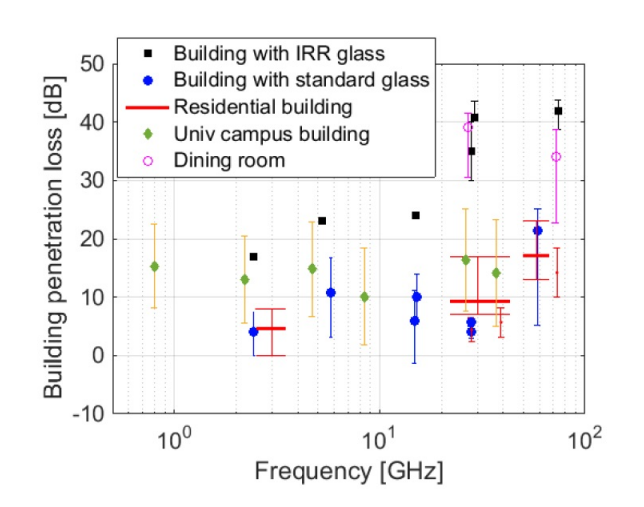
\includegraphics[width=\textwidth]{Fig1}
\caption{Attenuation due to outdoor to indoor penetration}
\end{figure}
Another case of attenuation caused by the same motives is the one caused by the shadowing of objects and people, which can cause losses of up to 20 dB.\par
\subsection*{5G data rates}
\paragraph{}
Besides the vulnerability to attenuation and pathloss, 5G still makes a solid step forward in data rate, being up to 1Tbps theoretically, though this volume is just expected to be achieved by 2030. Meanwhile, peak data rates over 10Gbps may be achieved in specific scenarios such as indoor and dense outdoor environments, in this case, A range of 10-50Gbps can be achieved for low mobility users, with ≥ 100Mbps cell-edge data rate guaranteed for 95% of the users [1].\par
Also, It is worth noting that the IMT-2020 has set minimum requirements for peak data rates in a workable 5G network to be 20Gbps and 10Gbps in the DL and UL respectively [1].\par
\subsection*{The future with 5G}
\paragraph{}
In the end, is important to notice the importance of the IoT inside the 5G key capabilities playing a pivotal role in enhancing living standards and production and service automation, once The trending 5 G-enabled IoT encompasses increased data rates, better coverage, and high throughput hence providing solutions to business models and leading to a world where everything is accessible on less time and effort[5].
\section

\section{Conclusion}
\paragraph*{} During this review it has been presented the step by steps of the principal revolutions and particularities of the evolution of data mobility and communication, through the advances in the 1G, 2G, 3G, 4G, and 5g, visiting the changes in protocols, data modulation, and data transmission methods and how they transformed the society, improving the amount and how fast data is transmitted, improving its stability and lowering latency, amplifying its range and making it accessible to the population.
\par No matter each one of the evolutions (1G...5G) is analyzed, it is indubitable that each one fully transformed the way the population and the industry related to the technology and administrated its communication, being caused by high hardware and software advances they still have needs to be addressed in the future such as problems in standardization and problems in transmission penetration, wich create ways to further improvements and evolutions in the future that may, again, change the way the society live.


\begin{thebibliography}{1}

\bibitem{}M.~Sonmez and A.~Akbal \emph{FPGA-Based BASK and BPSK Modulators Using VHDL:
Design, Applications and Performance Comparison for Different Modulator Algorithms}, International Journal of Computer Applications, 2012
\bibitem{}J.Sempere \emph{An overview of the GSM system} IEEE Vehicular Technology Society, 1999
\bibitem{}O.~Eluwole, N.~Udoh, M.~Ojo, C.~Okoro and A.~Akinyoade \emph{From 1G to 5G, What Next?} Hong Kong: IAENG International Journal of Computer Science, 2018
\bibitem{}M.~Shafi, A.~Molisch, P.~Smith, T.~Haustein, P.~Zhu, P.~Silva, F.~
Tufvesson, A.~Benjebbour, G.~Wunder\emph{5G: A Tutorial Overview of Standards, Trials, Challenges, Deployment and Practice"} IEEE Journal on Selected Areas in Communications, 2017
\bibitem{}K.~Shafique, B.~KHAWAJA, (Senior Member, IEEE), F~SABIR, S~QAZI, (Member, IEEE), M~MUSTAQIM \emph{Internet of Things (IoT) for Next-Generation Smart Systems: A Review of Current Challenges, Future Trends and Prospects for Emerging 5G-IoT Scenarios} IEEE Access, 2020
\end{thebibliography}

\begin{IEEEbiographynophoto}{André Melo}
Biography text here.
\end{IEEEbiographynophoto}

\begin{IEEEbiographynophoto}{Rafael Lima}
Biography text here.
\end{IEEEbiographynophoto}

% if you will not have a photo at all:
\begin{IEEEbiographynophoto}{Rodrigo Anciães}
Biography text here.
\end{IEEEbiographynophoto}

\end{document}